%%%%%%%%%%%%%%%%%%%%%%%%%%%%%%%%%%%%%%%%%
% Beamer Presentation
% LaTeX Template
% Version 1.0 (10/11/12)
%
% This template has been downloaded from:
% http://www.LaTeXTemplates.com
%
% License:
% CC BY-NC-SA 3.0 (http://creativecommons.org/licenses/by-nc-sa/3.0/)
%
%%%%%%%%%%%%%%%%%%%%%%%%%%%%%%%%%%%%%%%%%
%----------------------------------------------------------------------------------------
%	PACKAGES AND THEMES
%----------------------------------------------------------------------------------------
% Interessante: 
%https://www.codecogs.com/latex/eqneditor.php?lang=pt-br


\documentclass{beamer}

\usepackage[brazilian]{babel}
\usepackage[utf8]{inputenc}
\usepackage[T1]{fontenc}
\usepackage{colortbl}
\usepackage{mathrsfs}
\usepackage{smartdiagram}
\usepackage{listings}
\usepackage[framed,numbered,autolinebreaks,useliterate]{mcode}
\usepackage{multirow}
\usepackage{amssymb}
\usepackage{mdframed}


\mode<presentation> {

% The Beamer class comes with a number of default slide themes
% which change the colors and layouts of slides. Below this is a list
% of all the themes, uncomment each in turn to see what they look like.

%\usetheme{default}
%\usetheme{AnnArbor}
%\usetheme{Antibes}
%\usetheme{Bergen}
%\usetheme{Berkeley}
%\usetheme{Berlin}
%\usetheme{Boadilla}
%\usetheme{CambridgeUS}
%\usetheme{Copenhagen}
%\usetheme{Darmstadt}
%\usetheme{Dresden}
\usetheme{Frankfurt}
%\usetheme{Goettingen}
%\usetheme{Hannover}
%\usetheme{Ilmenau}
%\usetheme{JuanLesPins}
%\usetheme{Luebeck}
%\usetheme{Madrid}
%\usetheme{Malmoe}
%\usetheme{Marburg}
%\usetheme{Montpellier}
%\usetheme{PaloAlto}
%\usetheme{Pittsburgh}
%\usetheme{Rochester}
%\usetheme{Singapore}
%\usetheme{Szeged}
%\usetheme{Warsaw}

% As well as themes, the Beamer class has a number of color themes
% for any slide theme. Uncomment each of these in turn to see how it
% changes the colors of your current slide theme.

%\usecolortheme{albatross}
%\usecolortheme{beaver}
%\usecolortheme{beetle}
%\usecolortheme{crane}
%\usecolortheme{dolphin}
%\usecolortheme{dove}
%\usecolortheme{fly}
%\usecolortheme{lily}
%\usecolortheme{orchid}
%\usecolortheme{rose}
%\usecolortheme{seagull}
%\usecolortheme{seahorse}
%\usecolortheme{whale}
%\usecolortheme{wolverine}

%\setbeamertemplate{footline} % To remove the footer line in all slides uncomment this line
%\setbeamertemplate{footline}[page number] % To replace the footer line in all slides with a simple slide count uncomment this line

%\setbeamertemplate{navigation symbols}{} % To remove the navigation symbols from the bottom of all slides uncomment this line
}

\usepackage{graphicx} % Allows including images
\usepackage{booktabs} % Allows the use of \toprule, \midrule and \bottomrule in tables

\usepackage{animate}
\usepackage{hyperref}
\usepackage{media9}
\usepackage{listings}
\usepackage{amsmath}
\usepackage[framed,numbered,autolinebreaks,useliterate]{mcode}
\usepackage{chronology}
\usepackage{xpatch}
\xpretocmd{\chronology}{\tikzset{>=|}}{}{\failure}
\usepackage{mdframed}
\usepackage{tikz}
\usetikzlibrary{arrows.meta}
\tikzset{%
  >={Latex[width=2mm,length=2mm]},
  % Specifications for style of nodes:
         base/.style = {rectangle, rounded corners, draw=black,
                        minimum width=4cm, minimum height=0.7cm,
                        text centered, font=\sffamily},
         activityStarts/.style = {base, fill=blue!30},
         process/.style = {base, minimum width=2.5cm, fill=orange!15,
                          font=\ttfamily},
         ilumina/.style = {base, minimum width=2.5cm, fill=red!55,
                          font=\ttfamily},           
         coord/.style={coordinate, on chain, on grid, node distance=6mm and 25mm},
}

\usetikzlibrary{arrows,shapes,positioning,shadows,trees}

\tikzset{
  basic/.style  = {draw, text width=2cm, drop shadow, font=\sffamily, rectangle},
  root/.style   = {basic, rounded corners=2pt, thin, align=center,
                   fill=green!30},
  level 2/.style = {basic, rounded corners=6pt, thin,align=center, fill=green!60,
                   text width=8em},
  level 3/.style = {basic, thin, align=left, fill=pink!60, text width=6.5em}
}

%----------------------------------------------------------------------------------------
%	TITLE PAGE
%----------------------------------------------------------------------------------------

\logo
{
    
\includegraphics[width=0.6cm,height=0.6cm,keepaspectratio]{UFJF.jpg}~%
}

\title[Aula 2]{Programação Linear} 

\author
{
Prof. André Luís Marques Marcato \\
%\small andre.marcato@ufjf.edu.br
\href{mailto:andre.marcato@ufjf.edu.br}{\beamergotobutton{ andre.marcato@ufjf.edu.br }}
} % Your name

\institute[UFJF] % Your institution as it will appear on the bottom of every slide, may be shorthand to save space
{
Universidade Federal de Juiz de Fora \\

\includegraphics[width=1cm]{Engenharia.jpg} \\
}

%\date{\small \today} % Date, can be changed to a custom date
\date{\small Primeiro Semestre de 2018} % Date, can be changed to a custom date

\hypersetup{
    colorlinks=true,
    linkcolor=gray,
    filecolor=magenta,      
    urlcolor=cyan,
}

\begin{document}

\begin{frame}
\titlepage % Print the title page as the first slide
\begin{figure}[!htb]
\centering
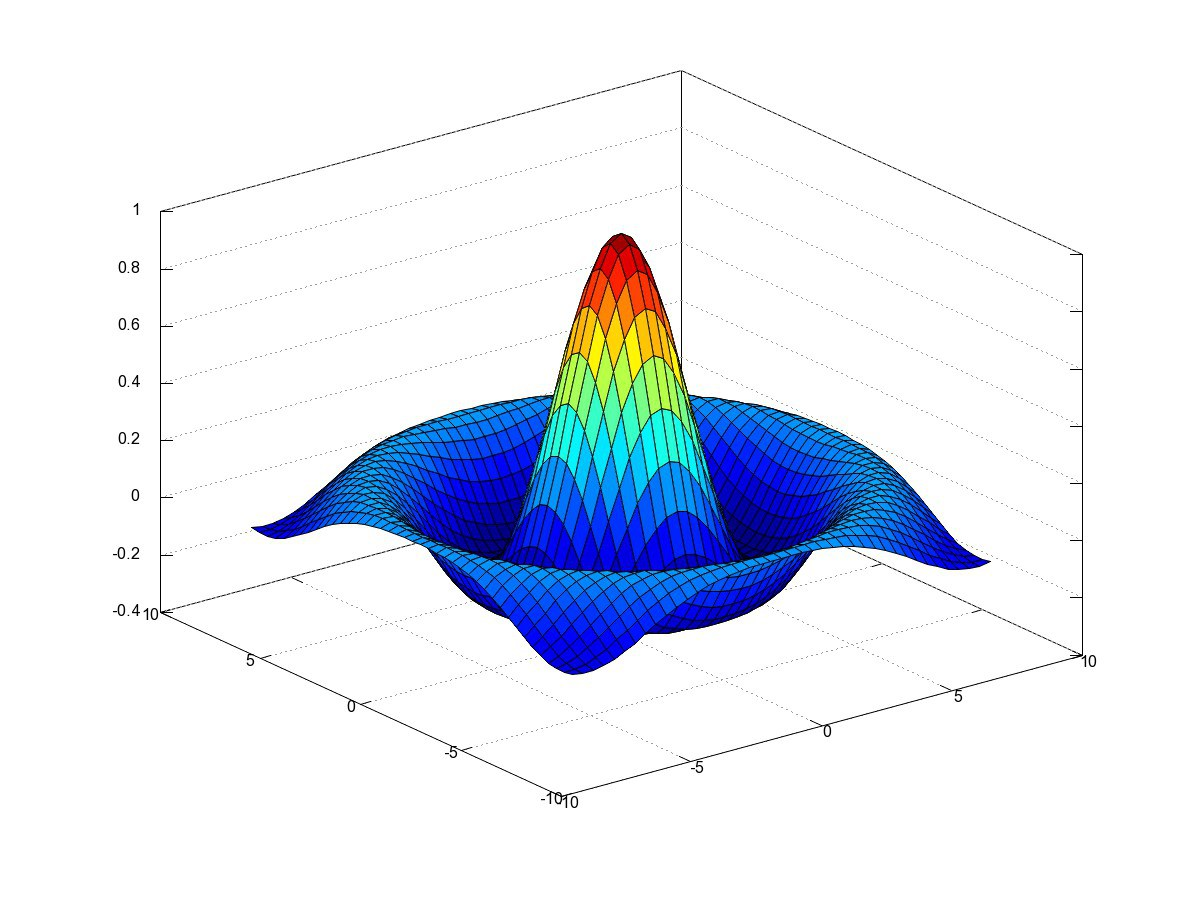
\includegraphics[width=2.6cm, height=1.7cm]{cover.jpg}
%\caption{Ogata - 5a Edicao - Fig. 1.1}
\label{Ogata_1_1}
\end{figure}
\end{frame}

\begin{frame}
\frametitle{Agenda da Apresentação} % Table of contents slide, comment this block out to remove it
\tableofcontents % Throughout your presentation, if you choose to use \section{} and \subsection{} commands, these will automatically be printed on this slide as an overview of your presentation
\end{frame}

%----------------------------------------------------------------------------------------
%	PRESENTATION SLIDES
%----------------------------------------------------------------------------------------

%\include{intro_e_avanco}

\section{Introdução}
\subsection{Histórico}

\begin{frame}
\frametitle{Histórico}
\centering
\begin{table}
	\begin{tabular}{c c}
	\only<1>{
				\multirow{5}{*}{\includegraphics[width=3cm,height=3cm]{fourier.jpg}} &
								Jean Baptiste Joseph Fourier (matemático \\ 
							  & Francês). Ele publicou um trabalho sobre a \\
							  & resolução de sistemas de equações lineares. \\
							  & Este trabalho é considerado o primeiro sobre \\
							  & programação linear. \\ 
				\multicolumn{2}{c}
				{
					\begin{chronology}[20]{1820}{2020}{\textwidth}
						\small
						\event{1827}{ {\color{red} 1827} - Fourier}
					\end{chronology} 
				} \\
			}
	\only<2>{
				\multirow{5}{*}{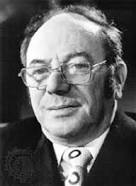
\includegraphics[width=3cm,height=3cm]{kantorovich.jpg}} &
								Leonide Kantorovich (matemático e economista \\ 
							  & Russo). Formulou e resolveu um problema de \\
							  & programação linear, mas seu trabalho permane- \\
							  & ceu desconhecido até 1959. \\
							  &  \\ 
				\multicolumn{2}{c}
				{
				\begin{chronology}[20]{1820}{2020}{\textwidth}
					\small
					\event[1939]{1959}{ {\color{red} 1939} - Kantorovich}
				\end{chronology} 
				} \\
			}
	\only<3>{
				\multirow{5}{*}{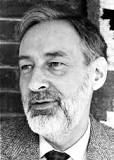
\includegraphics[width=3cm,height=3cm]{koopmans.jpg}} &
								O termo \alert{\underline{programação linear}} foi criado pelo   \\
							  & economista Holandês Tjalling Koopmans em \\
							  & uma conversa com Datzig na California  \\
							  & em 1948. Ele formulou modelos de progra- \\
							  & ção linear aplicados em economia clássica. \\ 
				\multicolumn{2}{c}
				{
				\begin{chronology}[20]{1820}{2020}{\textwidth}
					\small
					\event{1939}{ {\color{red} 1939} - Koopmans}
				\end{chronology} 
				} \\
			}
	\only<4>{
				\multirow{5}{*}{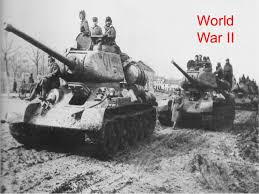
\includegraphics[width=3cm,height=3cm]{secondwar.jpg}} &
								Durante a Segunda Guerra Mundial, mode- \\
							  & los de programação linear foram  projetados \\
							  & e resolvidos em aplicações voltadas para  \\
							  & planejamento militar. \\
							  &  \\ 
				\multicolumn{2}{c}
				{
				\begin{chronology}[20]{1820}{2020}{\textwidth}
					\small
					\event[1939]{1945}{ {\color{red} Second War}}
				\end{chronology} 
				} \\
			}
	\only<5>{
				\multirow{5}{*}{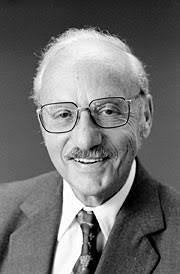
\includegraphics[width=3cm,height=3cm]{dantzig.jpg}} &
								Em 1947, George Dantzig desenvolveu o \\
							  & \alert{\underline{Método Simplex}}, propondo a Formulação \\ 
							  & Geral de Problemas de Programação Linear.  \\ 
							  & Ele trabalhava como  matemático consultor   \\
							  & para o Pentágono.\\ 
				\multicolumn{2}{c}
				{
				\begin{chronology}[20]{1820}{2020}{\textwidth}
					\small
					\event[1939]{1947}{ {\color{red} 1947} - Dantzig}
				\end{chronology} 
				} \\
			}			
	\only<6>{
				\multirow{5}{*}{
\includegraphics[width=3cm,height=3cm]{nobel.jpg}} &
								Em 1975, Kantorovich e Koopmans receberam   \\
							  & o Prêmio Nobel em Ciências Econômicas pelo \\
							  & trabalho desenvolvido na área de programação \\
							  & linear. \\
							  &  \\ 
				\multicolumn{2}{c}
				{
				\begin{chronology}[20]{1820}{2020}{\textwidth}
					\small
					\event{1975}{ {\color{red} 1975} - Prêmio Nobel}
				\end{chronology} 
				} \\
			}
	\only<7>{
				\multirow{5}{*}{
\includegraphics[width=3cm,height=3cm]{bitcoin.jpg}} &
								Atualmente, problemas de prog. linear   \\
							  & são resolvidos 1.000.000 de vezes mais \\
							  & rapidamente que 1985. Além disto, problemas  \\
							  & com mais de 1.000.000 variáveis e restrições \\
							  & são prontamente resolvidos.  \\ 
				\multicolumn{2}{c}
				{
				\begin{chronology}[20]{1820}{2020}{\textwidth}
					\small
					\event{2018}{ {\color{red} 2018} }
				\end{chronology} 
				} \\
			}			
\end{tabular}
\end{table}
\end{frame}

\begin{frame}
	\frametitle{Programação Linear - Histórico}
	\begin{itemize}
	\item[] {Os maiores problemas na resolução de PL na época}
		\begin{itemize}
		\only<1->
		{
		\item[] 
\includegraphics[width=0.5cm,height=0.2cm]{seta.png} Achar um ponto inicial, ponto de partida do algoritmo.
		} 
		\only<2->
		{
		\item[] 
\includegraphics[width=0.5cm,height=0.2cm]{seta.png} Reduzir a área de memória e o número de operações aritméticas sem causar limitações de uso.
		} 
		\only<3->
		{
		\item[] 
\includegraphics[width=0.5cm,height=0.2cm]{seta.png} Manter a precisão numérica para a obtenção de resultados significativos.
		} 
		\end{itemize}
	\only<4->
	{
	\item[] A partir de 1957, todos estes aspectos foram solucionados!
	} 
	\end{itemize}
\end{frame}

\subsection{Modelagem Matemática}

\begin{frame}
	\frametitle{Programação Linear - Modelagem Matemática}
	\begin{itemize}
	\item[] {Aspectos importantes para o levantamento do modelo:}
		\begin{itemize}
		\only<1->
		{
		\item[] 
\includegraphics[width=0.5cm,height=0.2cm]{seta.png} Identificação das variáveis;
		} 
		\only<2->
		{
		\item[] 
\includegraphics[width=0.5cm,height=0.2cm]{seta.png} Identificação dos objetivos.
		} 
		\only<3->
		{
		\item[] 
\includegraphics[width=0.5cm,height=0.2cm]{seta.png} Identificação dos aspectos restritivos.
		} 
		\end{itemize}
	\only<4->
	{
	\item[] O modelo é uma tentativa de representação da realidade e sua complexidade depende do grau de exatidão requerido.
	} 
	\end{itemize}
\end{frame}

\subsection{Exemplos}

\begin{frame}
	\frametitle{Programação Linear - Modelagem Matemática}
	\only<1>{
	\begin{columns}
		\begin{column}{0.7\textwidth}
			\centering
			\begin{exampleblock}{Exemplo 1}
				\scriptsize
				Um agricultor deseja cultivar duas variedades de cereais, \textbf{A} e \textbf{B}, em um área restrita a 100 ares ($100m^2$). Sendo que:
				\begin{itemize}
				\item 1 are do cereal \textbf{A} produz 8 sacas
				\item 1 are do cereal \textbf{B} produz 10 sacas
				\end{itemize}
				Para o plantio, cada cereal:
				\begin{itemize}
				\item Tipo \textbf{A} precisa de {\color{red} 3 homens-hora de trabalho por are}
				\item Tipo \textbf{B} precisa de {\color{red} 2 homens-hora de trabalho por are}
				\end{itemize}
				sendo que se dispõe até 240 homens-hora de trabalho para o cultivo e o custo da mão de obra é de \$200 (unidades monetárias) por homem-hora. \\~\\
				A demanda máxima é limitada pelo mercado a 480 sacas do cereal tipo \textbf{A}, vendido a \$150/saca, e 800 sacas do cereal \textbf{B}, vendido a \$120/saca. \\~\\
				O agricultor deseja otimizar a área de cultivo de forma a \alert{MAXIMIZAR O LUCRO}.
			\end{exampleblock}
		\end{column}
		\begin{column}{0.3\textwidth}
			\centering
			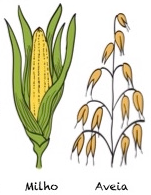
\includegraphics[width=2cm,height=3cm]{milho_aveia.png}
		\end{column}
	\end{columns}
	}
	\only<2>
	{
	\begin{columns}
		\begin{column}{0.7\textwidth}
			\centering
			\begin{exampleblock}{Exemplo 1 - As Variáveis do Problema}
				\scriptsize
				As variáveis estão relacionadas ao tamanho do terreno que será utilizado para o cultivo do cereal tipo \textbf{A} e \textbf{B}. Logo podemos definir;
				\begin{itemize}
				\item $x_1$: área destinada ao plantio do cereal Tipo \textbf{A}
				\item $x_2$: área destinada ao plantio do cereal Tipo \textbf{B} 
				\end{itemize}
			\end{exampleblock}
		\end{column}
		\begin{column}{0.3\textwidth}
			\centering
			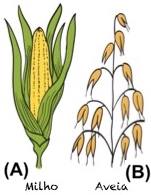
\includegraphics[width=2cm,height=3cm]{milho_aveia2.png}
		\end{column}
	\end{columns}	
	}	
	\only<3-7>
	{
	\begin{columns}
		\begin{column}{0.7\textwidth}
			\centering
			\begin{exampleblock}{Exemplo 1 - A Função Objetivo}
				\scriptsize
				Maximixar o lucro através da determinação ótima do tamanho do terreno que será utilizado para o cultivo dos cereais tipo \textbf{A} e \textbf{B}. \\~\\
				
				\begin{itemize}
				\item[]<4-> FOB = MAX LUCRO = MAX RECEITAS - CUSTOS
				\item<5-> $x_1$: Receitas: $receitas = \overset{\color{red}(150x8)}{1200}x_1+\overset{\color{red}(120x10)}{1200}x_2$
				\item<6-> $x_2$: Custos: $custos = \overset{\color{red}(200x3)}{600}x_1 + \overset{\color{red}(200x2)}{400}x_2$
				\item<7-> 
				$FOB = \max ({\color{red}600}x_1 + {\color{red}800}x_2)$ 
\includegraphics[width=1cm,height=1cm]{dinheiro2.jpg}
				\end{itemize}
			\end{exampleblock}
		\end{column}
		\begin{column}{0.3\textwidth}
			\centering
			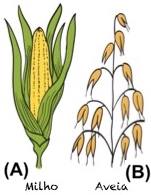
\includegraphics[width=2cm,height=3cm]{milho_aveia2.png}
		\end{column}
	\end{columns}	
	}
	\only<8-15>
	{
	\begin{columns}
		\begin{column}{0.7\textwidth}
			\centering
			\begin{exampleblock}{Exemplo 1 - As Restrições}
				\scriptsize
				\begin{itemize}
				\item<8-> {Desta forma a área custivada pelo cereal tipo \textbf{A} mais a área cultivada pelo cereal tipo \textbf{B} deve ocupar parte ou toda a área disponível de 100 ares}
					\begin{itemize}
					\item[$\circ$]<9->  $x_1+x_2 \le 100$
					\end{itemize}
				\item<10-> {Limitações de homem-hora}				
					\begin{itemize}
					\item[$\circ$]<11->  $3x_1+2x_2 \le 240$
					\end{itemize}
				\item<12-> {Limitações de devido à demanda de mercado}				
					\begin{itemize}
					\item[$\circ$]<13->  $8x_1 \le 480$ ou $x_1 \le 60$ para o cereal tipo \textbf{A}
					\item[$\circ$]<14->  $10x_2 \le 800$ ou $x_2 \le 80$ para o cereal tipo \textbf{B}
					\end{itemize}
				\end{itemize}
			\end{exampleblock}
		\end{column}
		\begin{column}{0.3\textwidth}
			\centering
			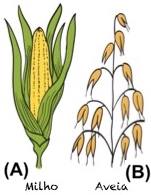
\includegraphics[width=2cm,height=3cm]{milho_aveia2.png}
		\end{column}
	\end{columns}
	}
	\only<16>
	{
	\begin{columns}
		\begin{column}{0.7\textwidth}
			\centering
			\begin{exampleblock}{Exemplo 1 - Modelo Matemático Completo}
				\scriptsize
				\begin{table}
					\begin{tabular}{r c l}
						$ \max Z = 600x_1+800x_2$ & 
\includegraphics[width=0.8cm,height=0.2cm]{seta2.png} & Função Objetivo \\
						sujeito a & & \\
						$x_1+x_2 \le 100$ & 
\includegraphics[width=0.8cm,height=0.2cm]{seta2.png}& Área Cultivo \\
						$3x_1+2x_2 \le 240$ & 
\includegraphics[width=0.8cm,height=0.2cm]{seta2.png}& Mão de Obra \\
						$x_1 \le 60 $ & 
\includegraphics[width=0.8cm,height=0.2cm]{seta2.png}& Produção Cereal \textbf{A} \\
						$x_2 \le 80 $ &
\includegraphics[width=0.8cm,height=0.2cm]{seta2.png} & Produção Cereal \textbf{B} \\
						$x_1, x_2 \ge 0$ & 
\includegraphics[width=0.8cm,height=0.2cm]{seta2.png}& Produção \\
					\end{tabular}
				\end{table}
			\end{exampleblock}
		\end{column}
		\begin{column}{0.3\textwidth}
			\centering
			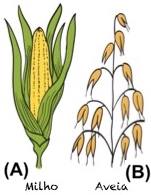
\includegraphics[width=2cm,height=3cm]{milho_aveia2.png}
		\end{column}
	\end{columns}	
	}
\end{frame}

\section{Solução Gráfica}
\subsection{Função Objetivo, Região Viável, Análise de Sensibilidade}

\begin{frame}
	\frametitle{Análise Gráfica} 
	\begin{columns}
		\begin{column}{0.5\textwidth}
			\centering
			\begin{exampleblock}{Exemplo 1 - Modelo Matemático}
				\scriptsize
				\begin{table}
					\begin{tabular}{r | l}
						{\color{red} $ \max Z = 600x_1+800x_2$ } & {\color{red} Objetivo } \\
						\only<10-22> 
						{
							sujeito a & \\
							{\color{blue}$x_1+x_2 \le 100$} &  {\color{blue} Área} \\
						}
						\only<12-22>
						{
							{\color{olive}$3x_1+2x_2 \le 240$} & {\color{olive}Mão de Obra} \\
						}
						\only<15-22>
						{
						{$x_1 \le 60 $ } & {Produção \textbf{A} } \\
						{$x_2 \le 80 $ } &  {Produção  \textbf{B} } \\
						{$x_1, x_2 \ge 0$ } &  {Produção } \\
						}
					\end{tabular}
				\end{table}
			\end{exampleblock}
			\only<22>
			{
			    \begin{mdframed}[backgroundcolor=blue!20] 
					Solução Ótima: $X_1 = 20$ e $X_2 = 80$ !!!
			    \end{mdframed}			
			}
		\end{column}
		\begin{column}{0.5\textwidth}
			\centering
			\only<1> {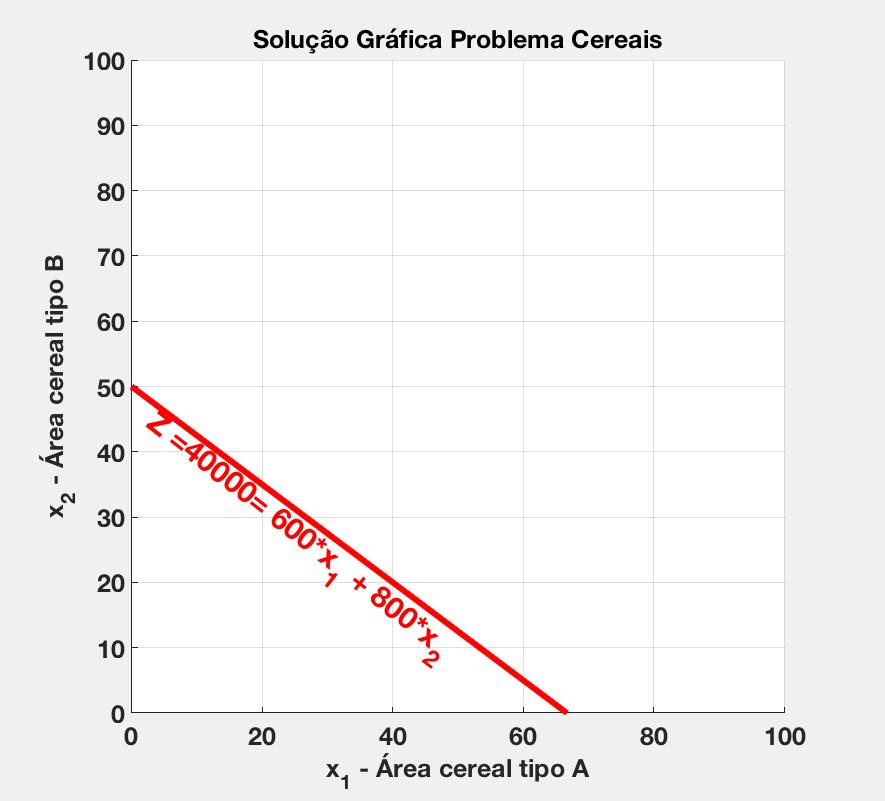
\includegraphics[width=6cm,height=6cm]{MatLab/anima_1.png} }
			\only<2> {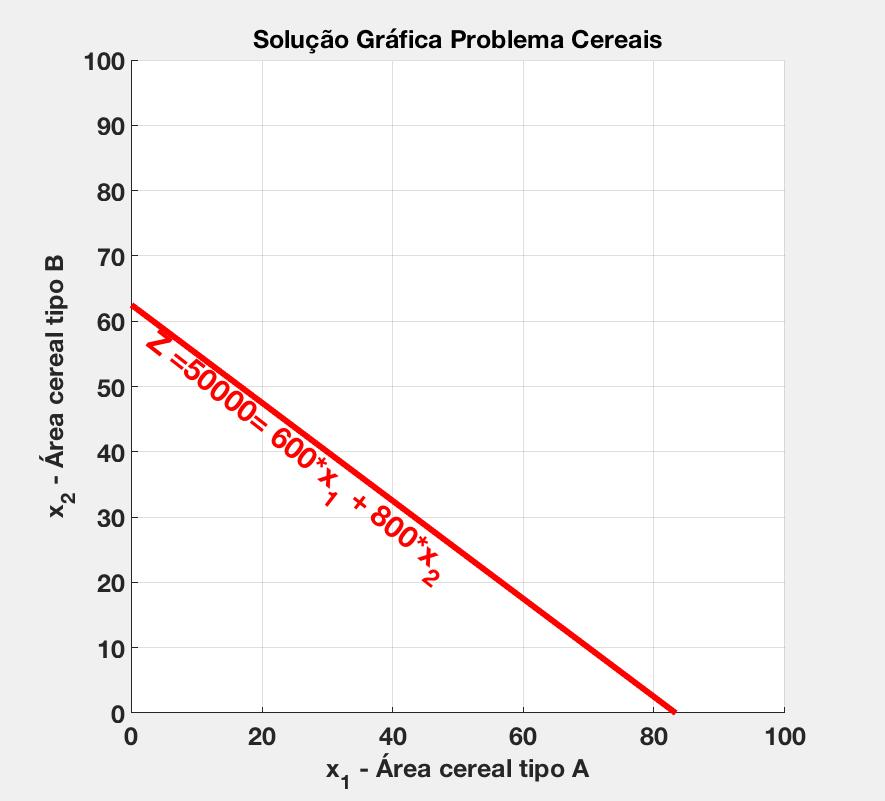
\includegraphics[width=6cm,height=6cm]{MatLab/anima_2.png} }
			\only<3> {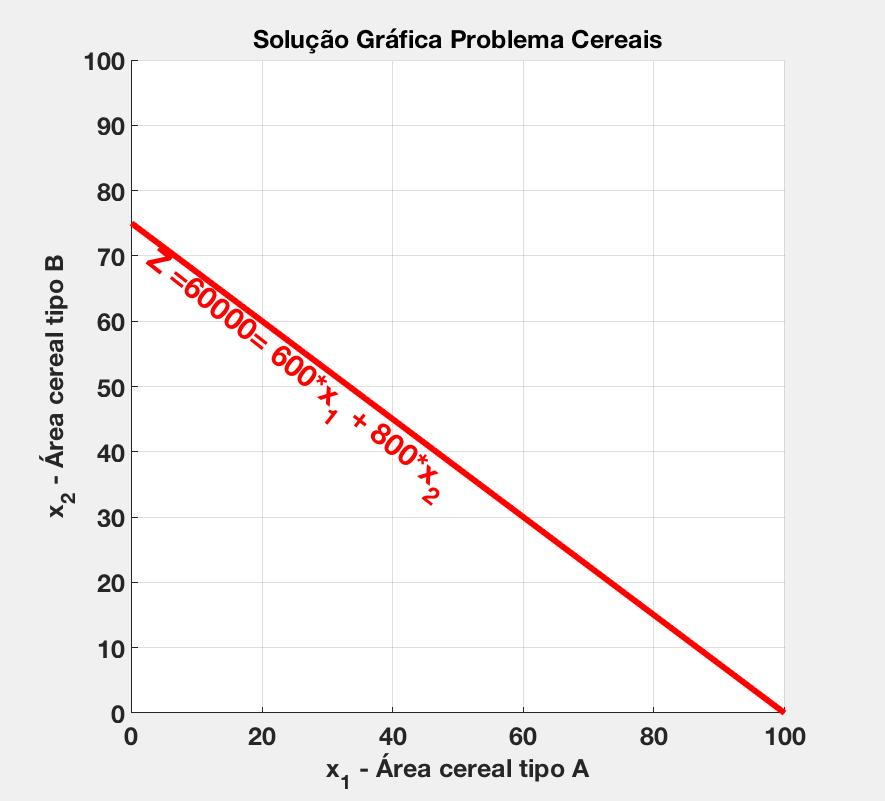
\includegraphics[width=6cm,height=6cm]{MatLab/anima_3.png} }
			\only<4> {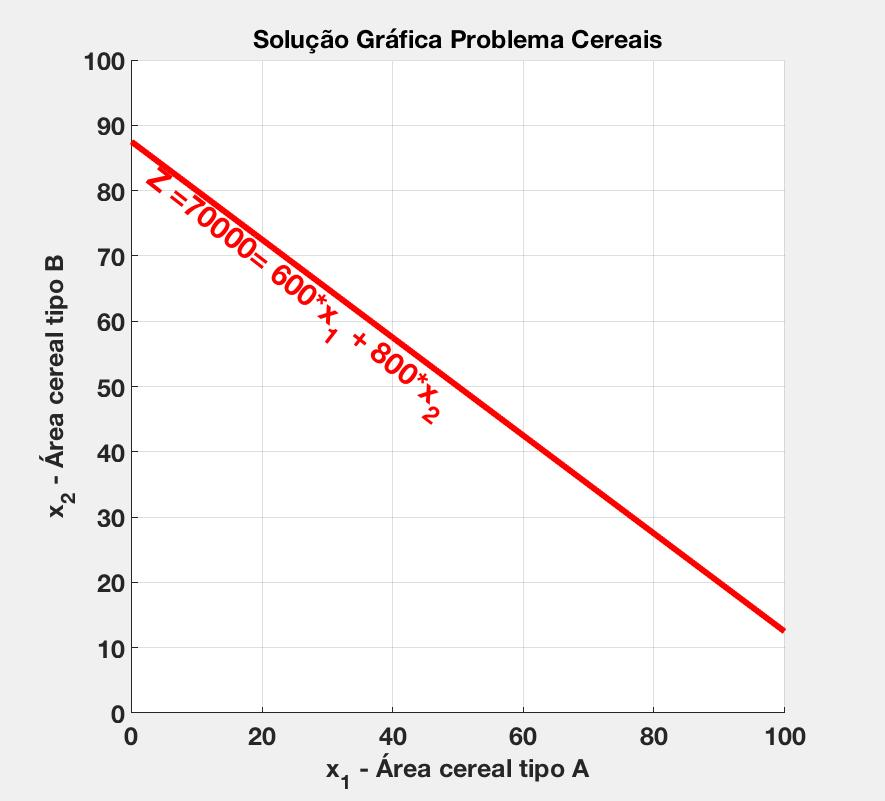
\includegraphics[width=6cm,height=6cm]{MatLab/anima_4.png} }
			\only<5> {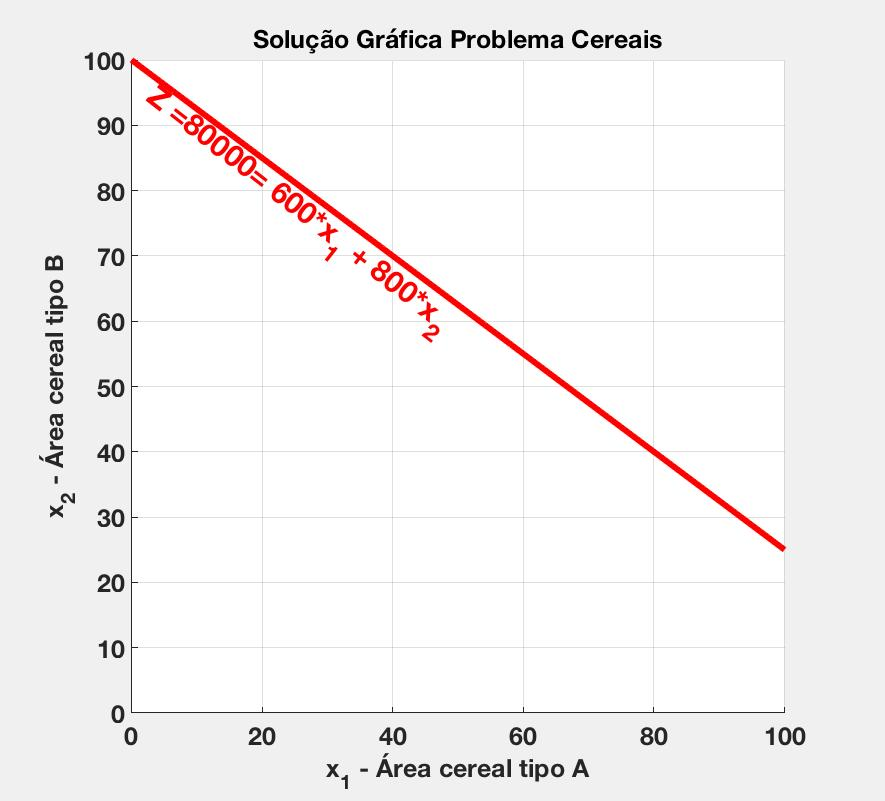
\includegraphics[width=6cm,height=6cm]{MatLab/anima_5.png} }
			\only<6> {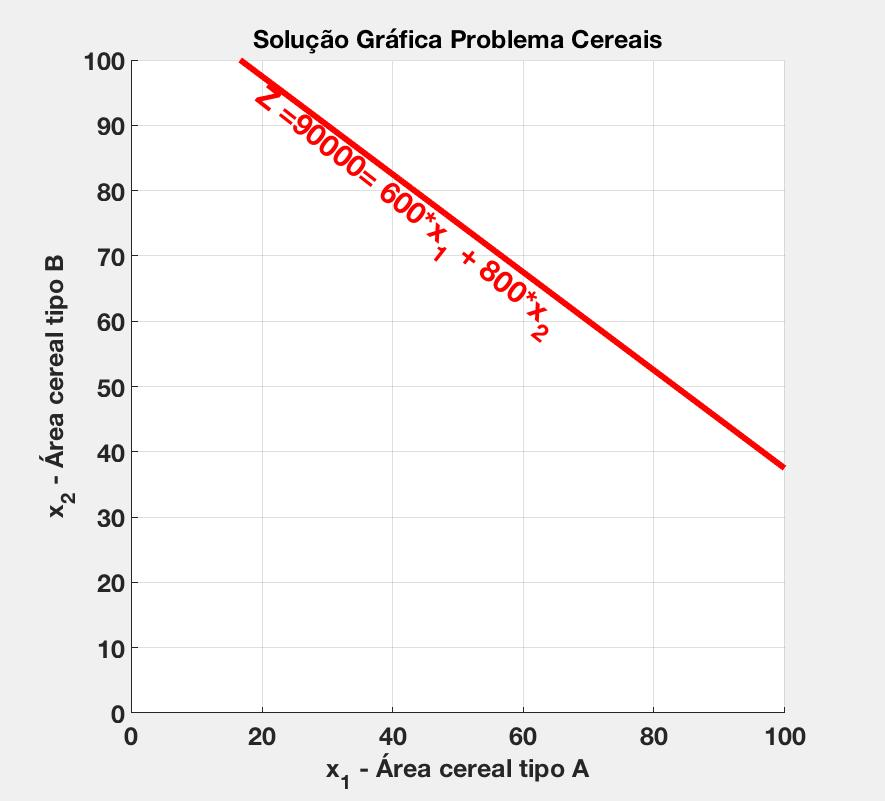
\includegraphics[width=6cm,height=6cm]{MatLab/anima_6.png} }
			\only<7> {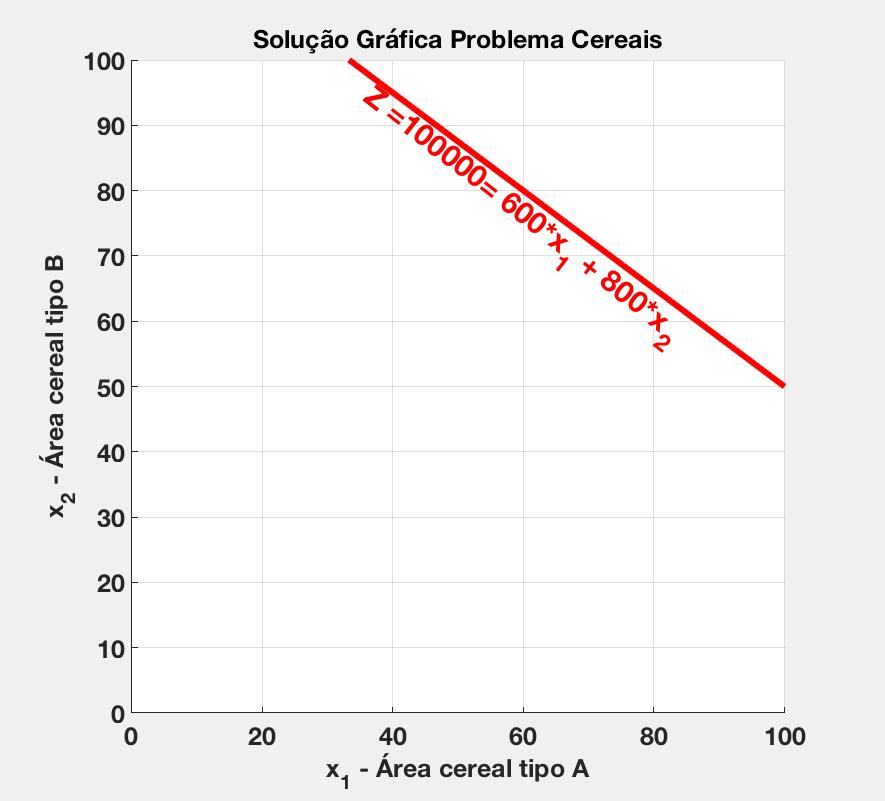
\includegraphics[width=6cm,height=6cm]{MatLab/anima_7.png} }
			\only<8> {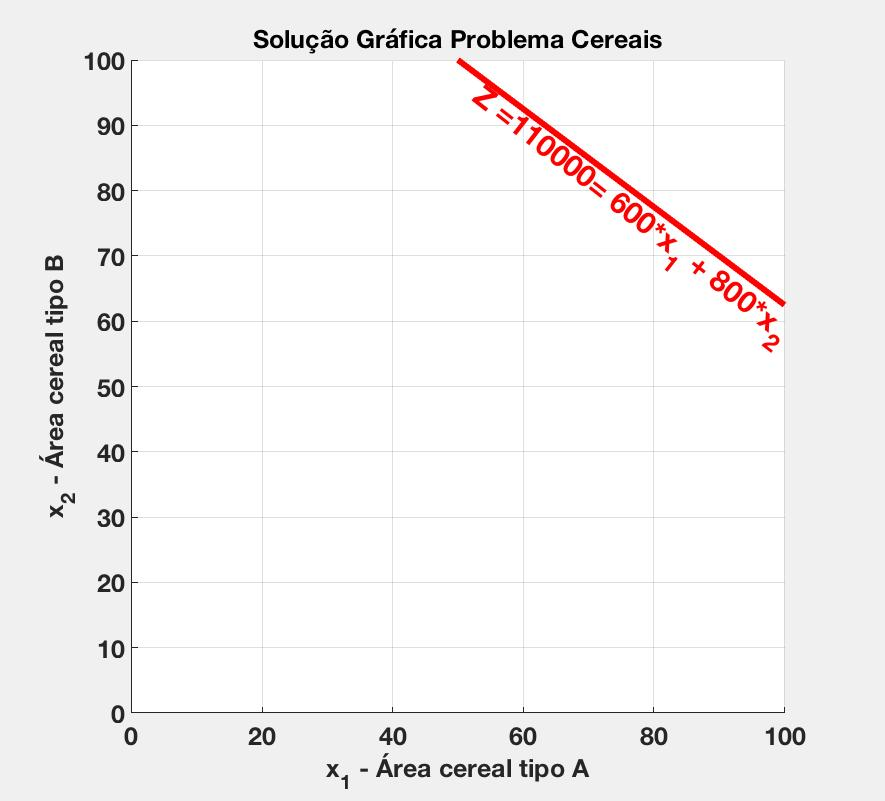
\includegraphics[width=6cm,height=6cm]{MatLab/anima_8.png} }
			\only<9-10> {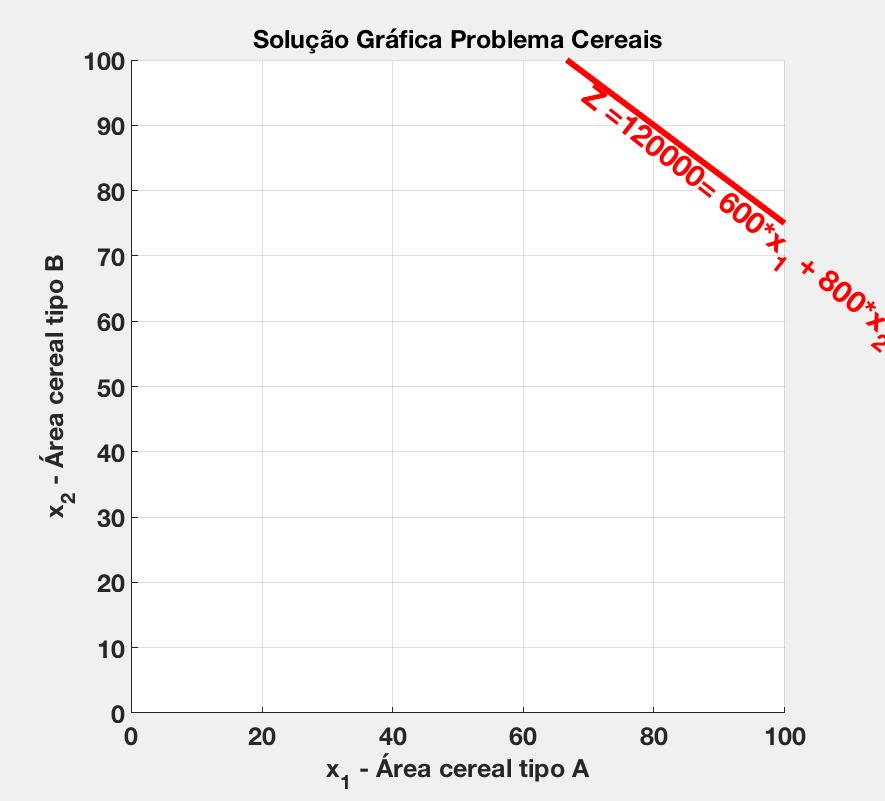
\includegraphics[width=6cm,height=6cm]{MatLab/anima_9.png} }
			\only<11-12> {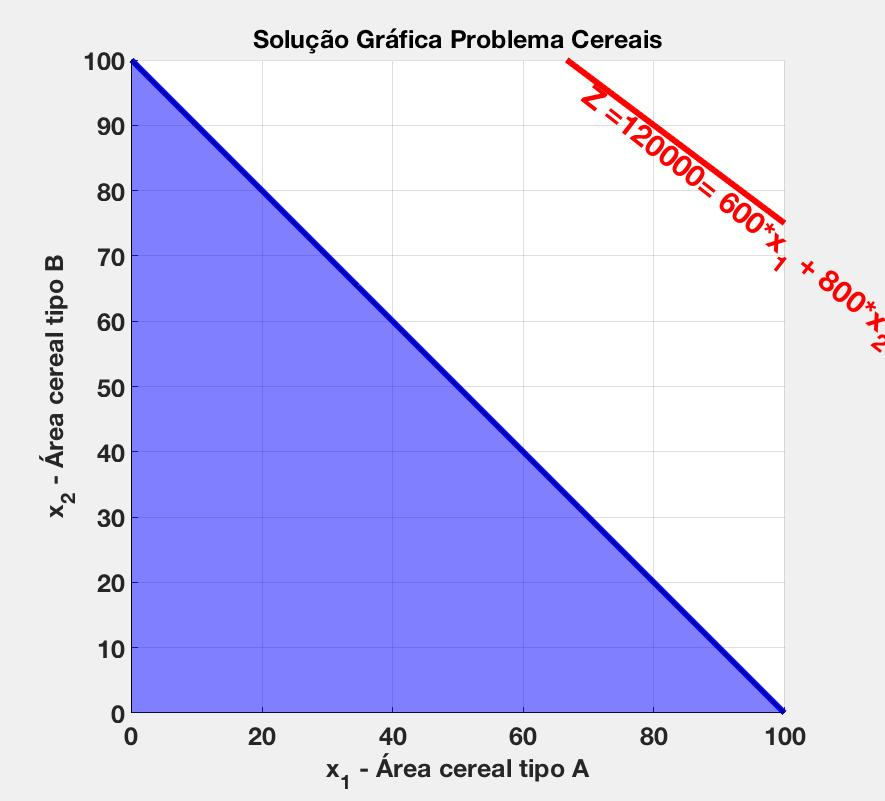
\includegraphics[width=6cm,height=6cm]{MatLab/anima_10.png} }
			\only<13> {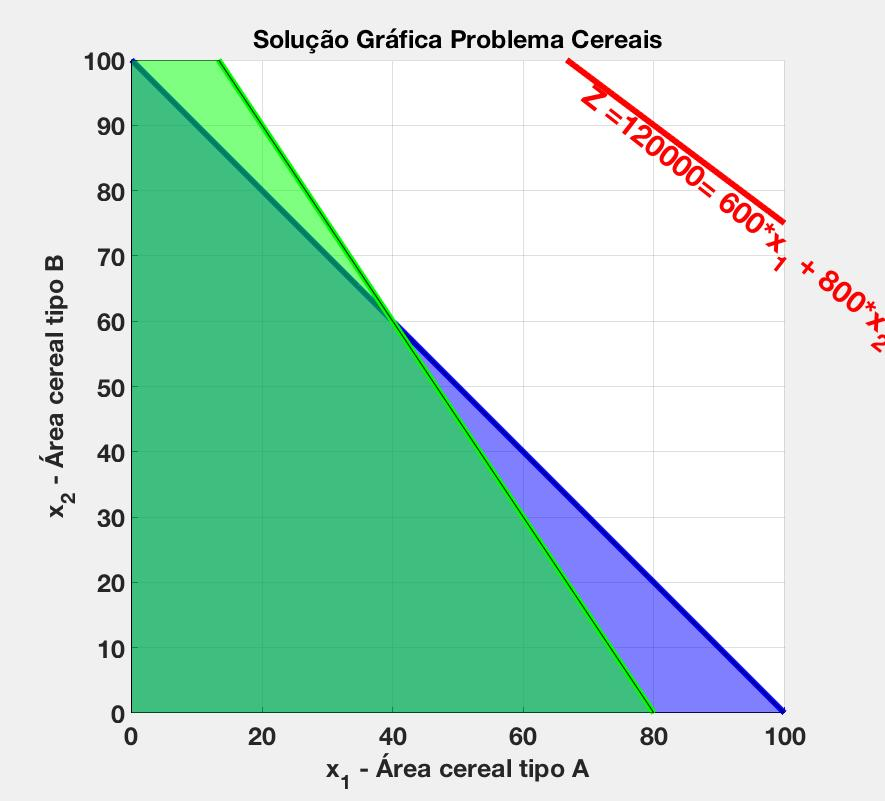
\includegraphics[width=6cm,height=6cm]{MatLab/anima_11.png} }
			\only<14-15> {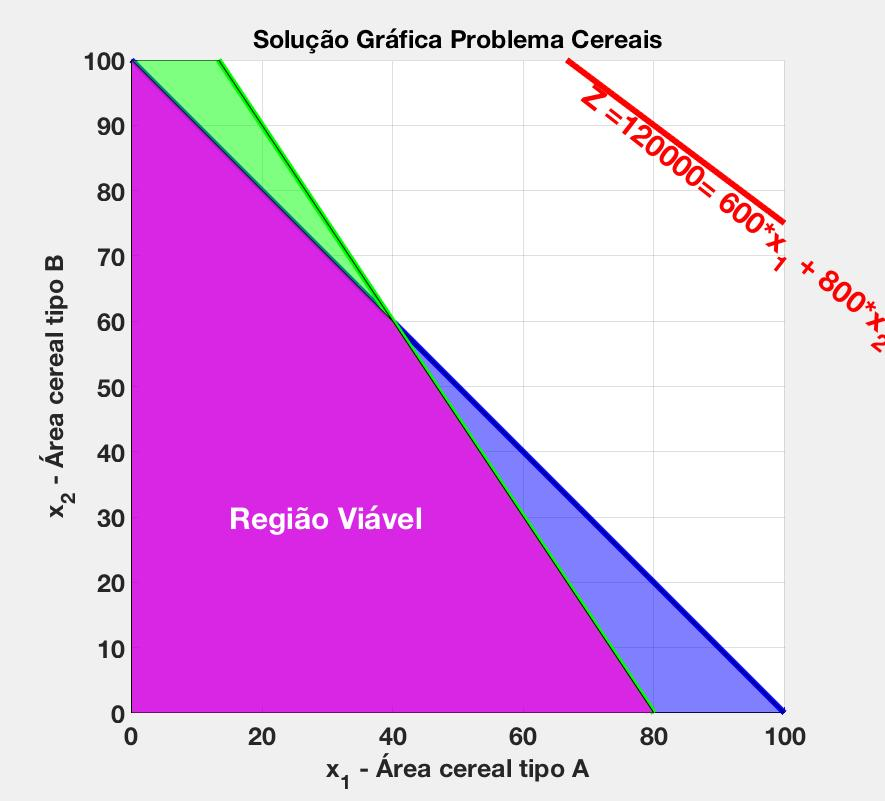
\includegraphics[width=6cm,height=6cm]{MatLab/anima_12.png} }
			\only<16> {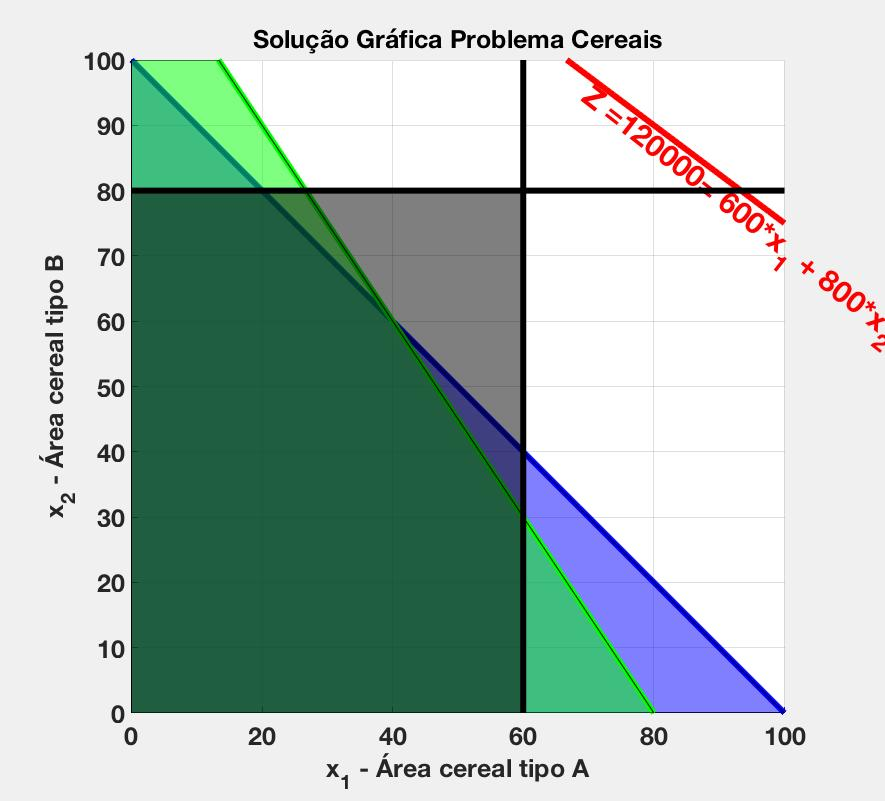
\includegraphics[width=6cm,height=6cm]{MatLab/anima_13.png} }
			\only<17> {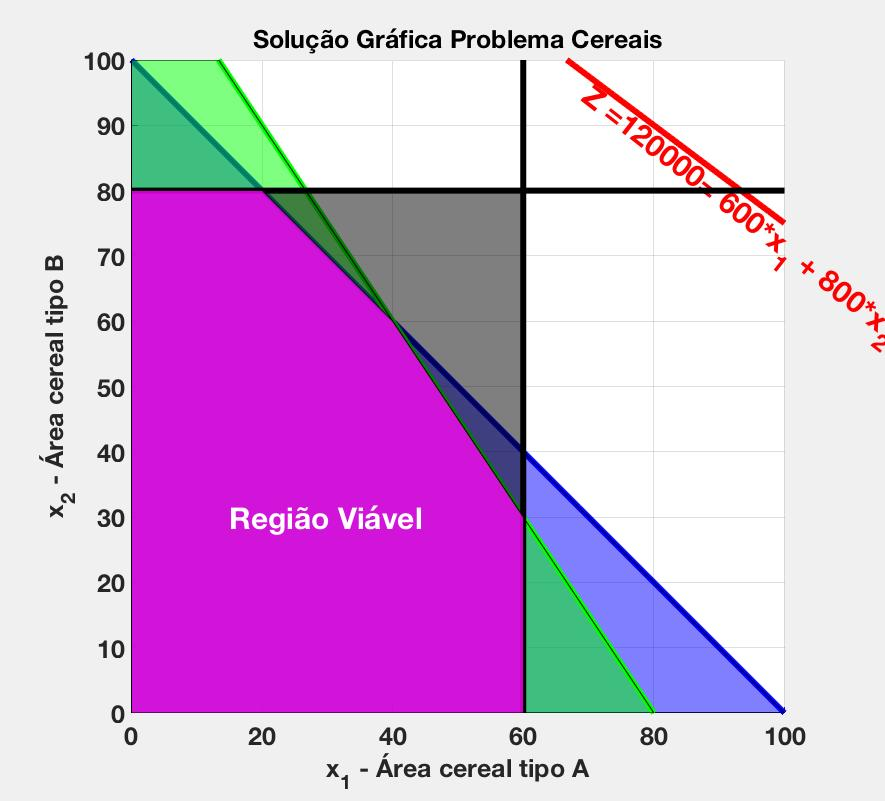
\includegraphics[width=6cm,height=6cm]{MatLab/anima_14.png} }
			\only<18> {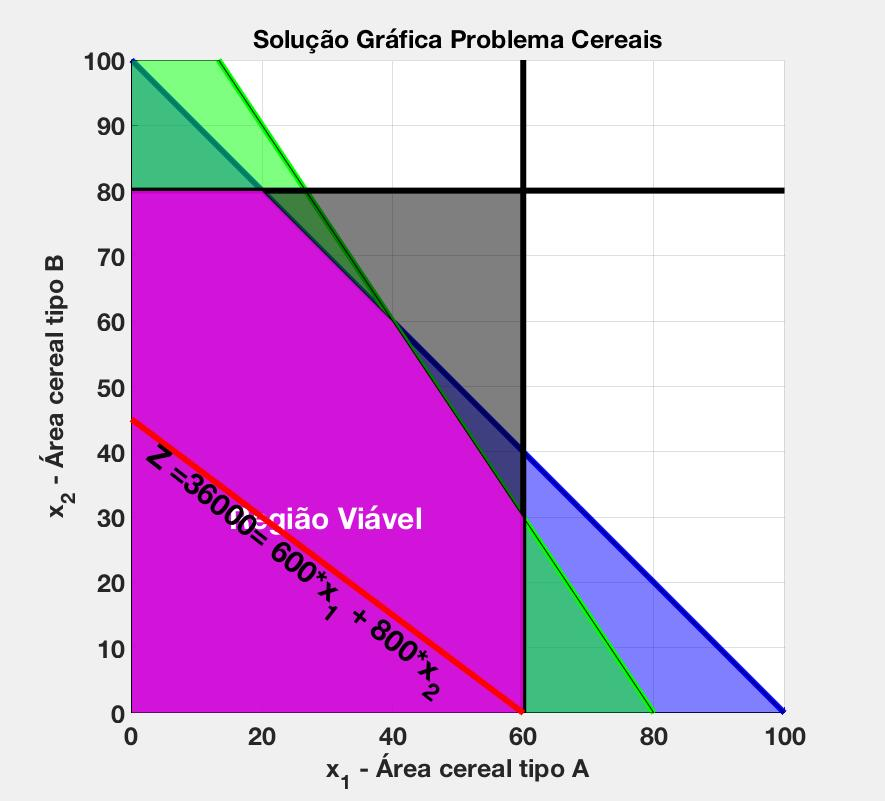
\includegraphics[width=6cm,height=6cm]{MatLab/anima_15.png} }
			\only<19> {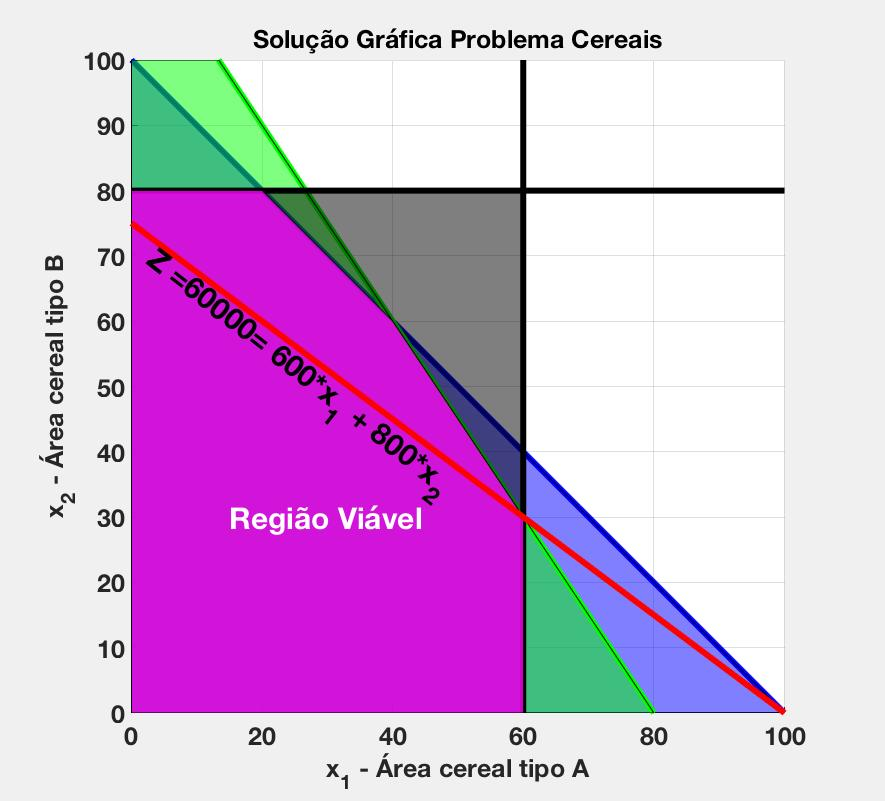
\includegraphics[width=6cm,height=6cm]{MatLab/anima_16.png} }
			\only<20> {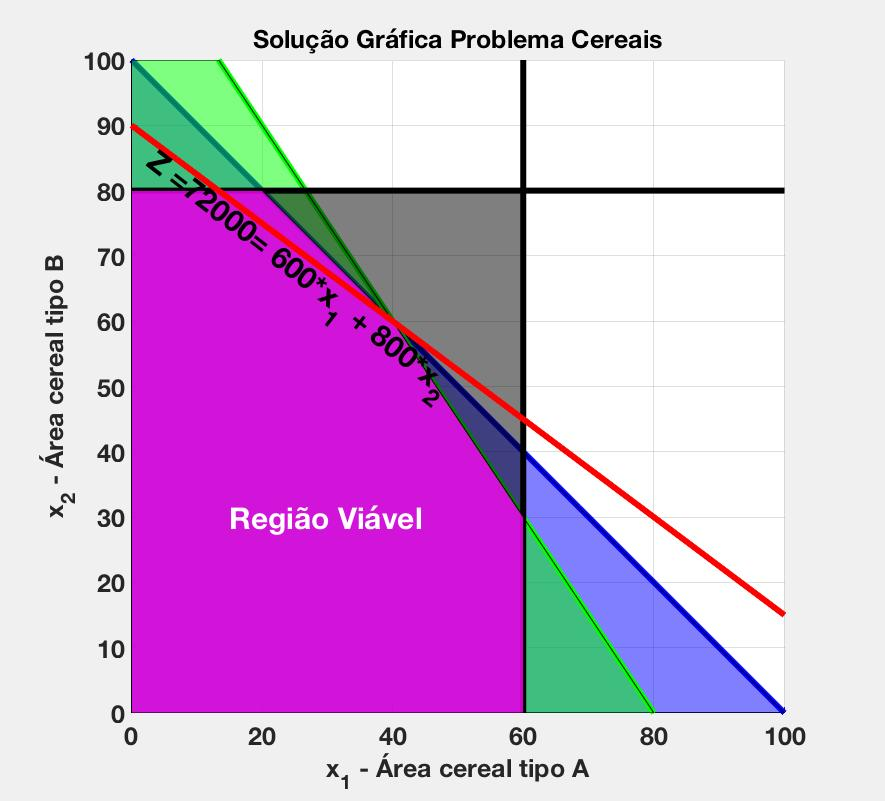
\includegraphics[width=6cm,height=6cm]{MatLab/anima_17.png} }
			\only<21-22> {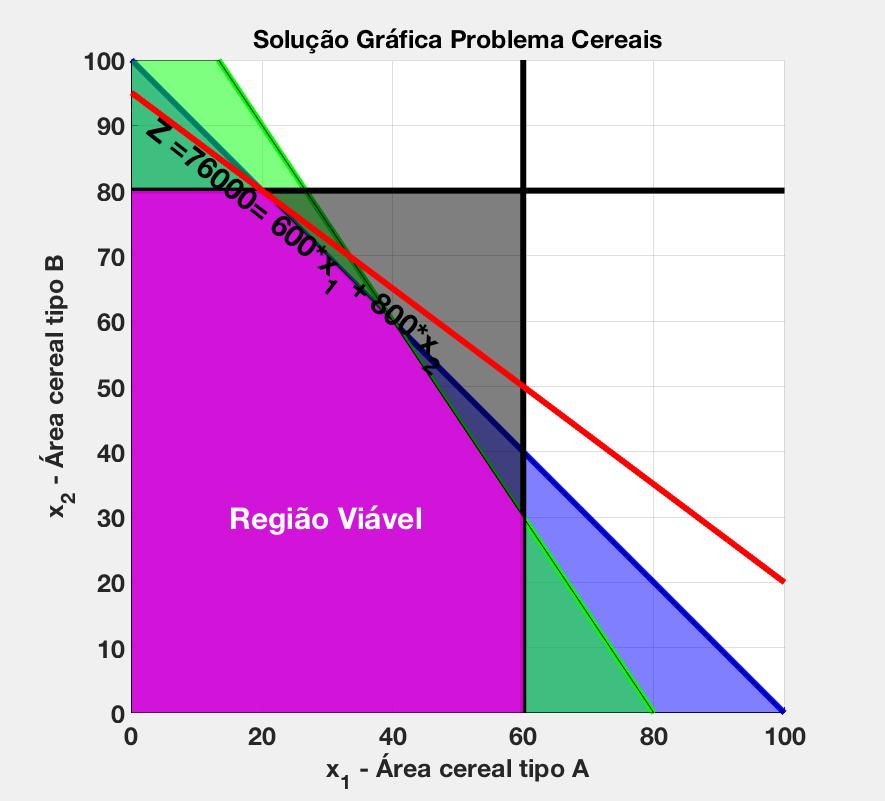
\includegraphics[width=6cm,height=6cm]{MatLab/anima_18.png} }
		\end{column}
	\end{columns}		
\end{frame}

\section{Formulação Matricial}
\subsection{c, A, B, Aeq, Beq, lowerbound, upper bound}


\begin{frame}
\Huge{\centerline{Fim}}
\end{frame}

%----------------------------------------------------------------------------------------

\end{document} 